\documentclass[pra,superscriptaddress,reprint,showpacs]{revtex4-1}
\usepackage[per-mode=symbol]{siunitx}   
\usepackage{comment} 
\usepackage{amssymb}
\usepackage{fancyhdr}
\usepackage{titlesec}
\usepackage{physics}
\usepackage{xcolor}
\usepackage{tikz}
\usepackage{lipsum}
\usepackage{float}
\usepackage{gensymb}
\usepackage{enumitem}
\usepackage{siunitx}
\usepackage{fourier}
\usepackage{arydshln}
\usepackage{csvsimple}
\usepackage{mathtools}
\usepackage{booktabs}
\usepackage[section]{placeins}
\usepackage{fancyvrb}
\usepackage{listings}
\usepackage{color}
\usepackage[cache=false]{minted}

\definecolor{bg}{rgb}{0.95,0.95,0.95}
\setminted[java]{breaklines=true}

\definecolor{dkgreen}{rgb}{0,0.6,0}
\definecolor{gray}{rgb}{0.5,0.5,0.5}
\definecolor{mauve}{rgb}{0.58,0,0.82}

\lstset{frame=tb,
  language=Java,
  aboveskip=3mm,
  belowskip=3mm,
  showstringspaces=false,
  columns=flexible,
  basicstyle={\small\ttfamily},
  numbers=none,
  numberstyle=\tiny\color{gray},
  keywordstyle=\color{blue},
  commentstyle=\color{dkgreen},
  stringstyle=\color{mauve},
  breaklines=true,
  breakatwhitespace=true,
  tabsize=3
}
\titleformat{\section}{\bf \center\uppercase}{\thesection}{1em}{}
\titleformat{\subsection}{\bf \center}{Part \thesubsection.}{1em}{}
\begin{document}
\title{Homework Assignment 4}
\date{\today}
\author{Dillon Peterson}
\email[send correspondence to: ]{dillonlpeterson@tamu.edu}
\affiliation{Department of Physics and Astronomy, Texas A\&M University,
College Station, TX. ~~77845}

\pacs{23.23.+x, 56.65.Dy}
\maketitle

\section{Problem 1}
\begin{center}
\checkmark
\end{center}

\section{Problem 2}
\subsection{}
\begin{figure}[h!]
    \centering
    \caption{10 Periods}
    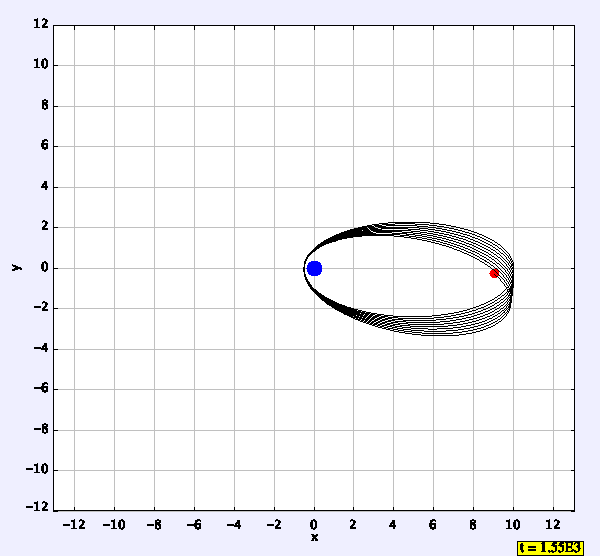
\includegraphics[width=7cm]{2aa.png}
\end{figure}

\subsection{}
When we set $nspeed=759$, the orbit starts to undergo highly pronounced precession. 

\begin{figure}[H]
    \centering 
    \caption{6 O'Clock}
    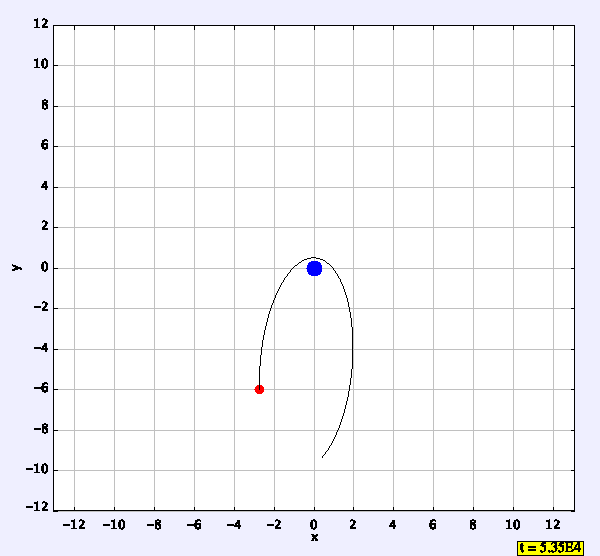
\includegraphics[width=7cm]{6oclock.png}
\end{figure}

\section{Problem 3}

\begin{figure}[H]
    \centering 
    \caption{Closed Orbit}
    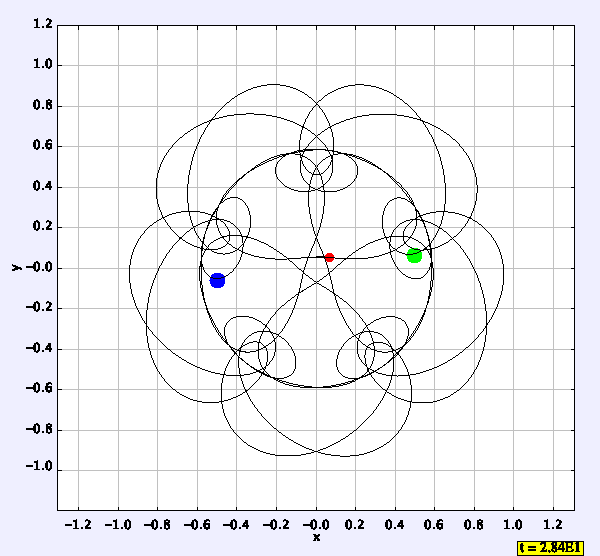
\includegraphics[width=7cm]{3.png}
\end{figure}

The period of the orbit is approximately \boxed{\approx\SI{28.4}{\s}}

\section{Problem 4}

\begin{figure}[h!]
    \centering 
    \caption{Closed Orbit (Co-Rotating Frame)}
    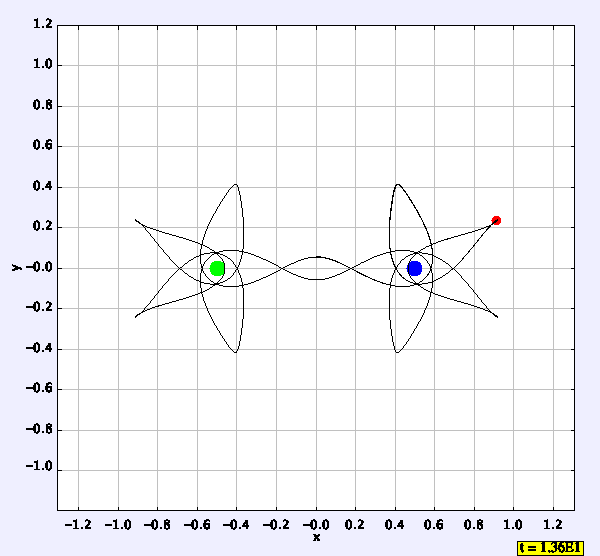
\includegraphics[width=7cm]{corot.png}
\end{figure}

\section{Problem 5}
\begin{figure}[h!]
    \centering 
    \caption{Chaotic Closed Orbit (Rotating Frame)}
    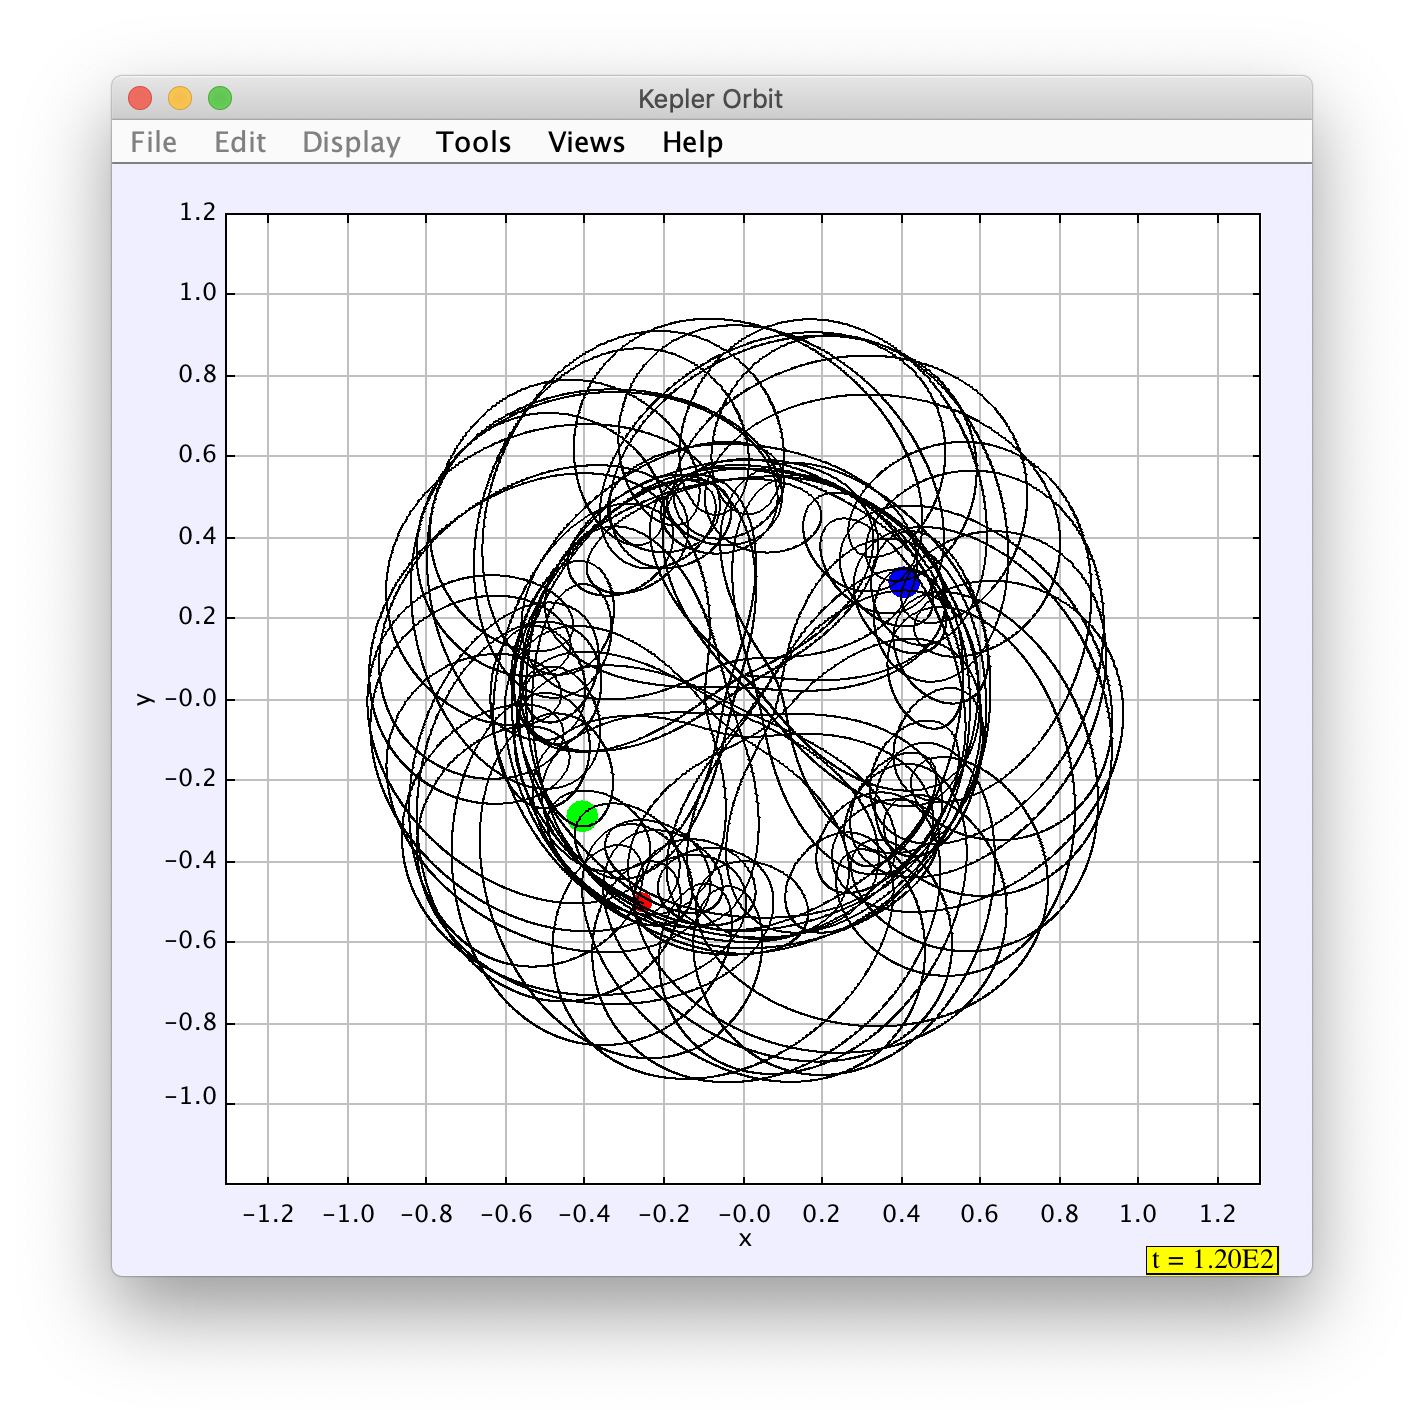
\includegraphics[width=7cm]{5chaoticorbit.png}
\end{figure}

\begin{figure}[h!]
    \centering 
    \caption{Chaotic Closed Orbit Input Parameters}
    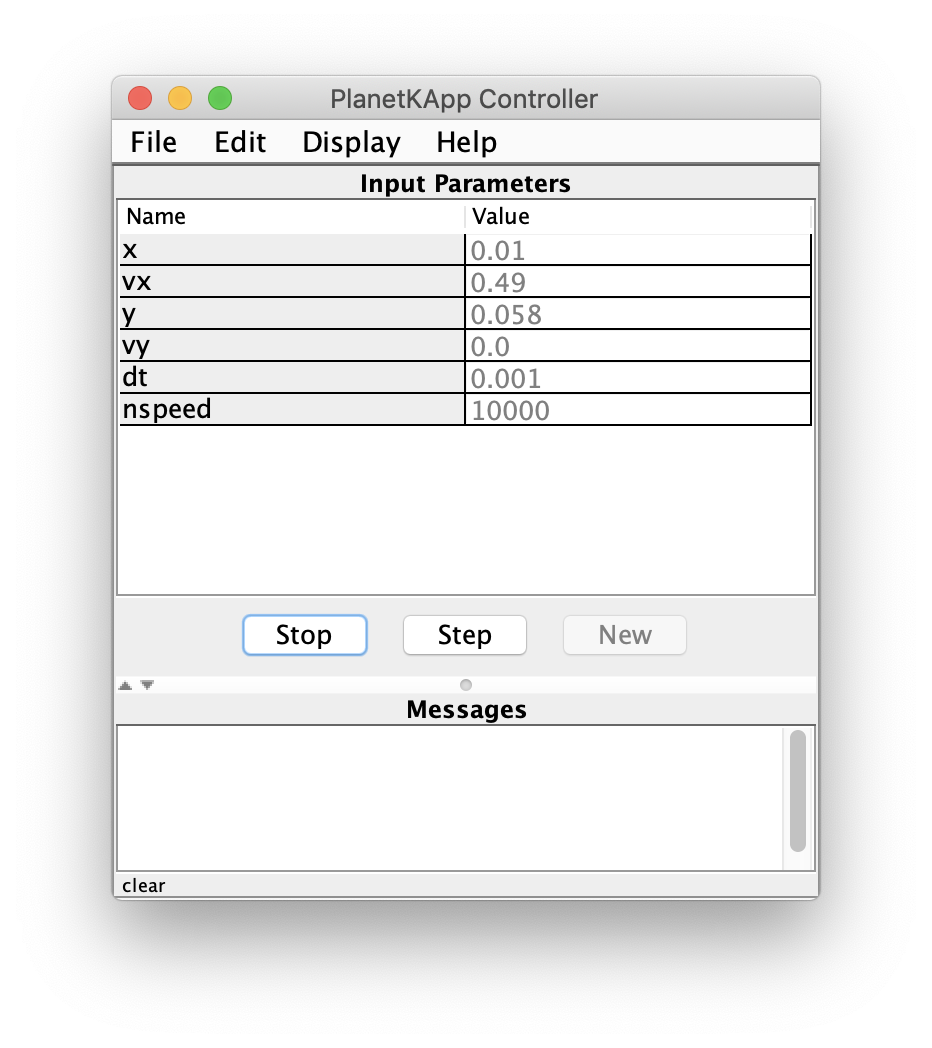
\includegraphics[width=7cm]{5ip.png}
\end{figure}

\end{document}



